\documentclass[a4paper,man,natbib,floatsintext,donotrepeattitle]{apa6}

\usepackage[english]{babel}
\usepackage[utf8x]{inputenc}
\usepackage{amsmath}
\usepackage{graphicx}
\usepackage[colorinlistoftodos]{todonotes}
\usepackage{xcolor}
\usepackage[draft,inline,nomargin,index]{fixme}
\usepackage[hidelinks]{hyperref}
\usepackage{verbatim}
\usepackage{nameref}
\usepackage{booktabs}
\usepackage{lineno}
\usepackage{amsfonts}
\usepackage{booktabs}
\usepackage{siunitx}
\newcommand*{\doi}[1]{\href{http://dx.doi.org/#1}{ #1}}
\linenumbers

\fxsetup{theme=color,mode=multiuser}
\FXRegisterAuthor{ab}{sab}{\color{blue}Amelie} % abnote{} with text inside to edit
\FXRegisterAuthor{bb}{sbb}{\color{purple}Brice} % bbnote{} with text inside to edit
\FXRegisterAuthor{ln}{sln}{\color{violet}Lad} % lnnote{} with text inside to edit

\title{Automation in Sequential Testing: A commentary on \cite{schonbrodt_sequential_2017}}

\shorttitle{Blind Bayes Factor}
\threeauthors{Amélie Bret}{Brice Beffara}{Ladislas Nalborczyk}
\threeaffiliations{Univ. Grenoble Alpes, CNRS, LPNC, 38000 Grenoble, France \\ Psychological Science Research Institute, Catholic University of Louvain, Belgium \\ The Walden III Slowpen Science Laboratory, France}{The Walden III Slowpen Science Laboratory, Villeurbanne, France}{Department of Experimental Clinical and Health Psychology, Ghent University \\ The Walden III Slowpen Science Laboratory, Villeurbanne, France }

\abstract{In this article we discuss the use of the Sequential Bayes Factor (SBF) procedure as introduced by \cite{schonbrodt_sequential_2017} when confronted with real world data, which contrary to simulated data can be complicated to handle. For example, when fitting a model to real world data several choices must be made to ensure that subsequent model comparisons are sensible. The SBF procedure itself is expected to inform us about the adequate sample size to reach a conclusion based on sequential accumulating data. Accordingly, we suggest that one should also prepare the data in a sequential way before computing a Bayes Factor. We propose a full automation procedure, in line with the preregistration philosophy and allowing analyses blinding. We provide recommendations on how to implement this  without additional costs, while taking into account the specificity of the sequential testing situation.}

\keywords{Sequential Bayes Factor, sequential testing, automation, preregistration, blind analyses}

\begin{document}

% defining a new command for counting words
\newcommand{\quickwordcount}{%
  \immediate\write18{texcount -1 -sum -merge \jobname.tex > \jobname-words.sum }%
  \input{\jobname-words.sum}words%
}

\maketitle

Wordcount: This document contains \textbf{\quickwordcount}.

\newpage

\section{Introduction}

\cite{edwards_bayesian_1963} state, "the rules governing when data collection stops are irrelevant to data interpretation. It is entirely appropriate to collect data until a point has been proven or disproven, or until the data collector runs out of time, money, or patience". However, this practice has severe pitfalls in the classical Null Hypothesis Significance Testing (NHST) paradigm, as it dramatically increases Type I error rates \citep[but see][]{lakens_performing_2014}.

In their paper, \cite{schonbrodt_sequential_2017} present an alternative to NHST with a priori power analysis (NHST-PA) by introducing the \textit{Sequential Bayes Factor} (SBF). The SBF allows for iterative data collection up until a predefined threshold and does not suffer from the pitfalls associated with NHST-PA. Testing mean differences between two independent groups, they show that the SBF design typically needs 50\% to 70\% smaller samples to reach a conclusion about the presence of an effect, as compared with optimal NHST-PA (where \textit{optimal} stands for an idealised situation in which the a priori targeted effect would be exactly equal to the population effect size), with both analyses showing similar long-term error rates.

The procedure described in \cite{schonbrodt_sequential_2017} offers an attractive perspective on data collection and we generally agree with most of their recommendations. However, we would draw attention to precautions that need to be undertaken in order to preserve the long-term rates of wrong inference they provide. One major concern is that when dealing with real-world data many analysis choices can be made before comparing models (i.e., before computing a Bayes Factor). Depending on the type of data researchers might have to decide upon signal processing methods, the rejection of outliers and other potential prerequisites. Dealing with these choices without optionally stopping data collection entails that the data analyst should not interact with data during data collection. Hence, all these decisions have to be made and implemented beforehand. To this end, we propose a fully automatised sequential procedure from data extraction to model comparison. The procedure is embedded in the preregistration philosophy and in addition gives certain methodological advantages. 

\section{Intrapersonal biases in SBF procedure}

When a data analyst has expectations about what should be observed, data analysis is likely to be biased by these expectations through confirmation (favoring an hypothesis) or disconfirmation (stronger skepticism toward data against the hypothesis than toward data corroborating the hypothesis) biases \citep{lilienfeld_blind_2017}.
When sequentially computing a Bayes Factor (BF), we are faced with many choices about how to deal with new incoming data. Based on previous studies, we might have expectations about the range of plausible values, particular methods to process physiological signals, the need for recoding or transforming data, or the distribution of residuals, and so on. We propose that these decisions should be made before starting the SBF procedure.

The SBF procedure has been validated based on simulated data \citep{schonbrodt_sequential_2017}. However, noise and irregularities in simulated data can only come from sampling variability, and not from practical problems encountered during empirical data collection (e.g., participant or experimenter errors). When dealing with real world data, we would like to get as close as possible to the shape of simulated data (i.e., we would like to minimise other sources of errors than sampling variability). In order for the Bayes Factor to be a reliable stopping criterion, it has to be computed on reliable data. What is considered \textit{reliable} data is conditional on the type of study, and should be justified by the existing literature as much as possible. However, changing the criterion and methods for data preparation based on some states of the SBF procedure is not acceptable. This implies that i) the researcher is well aware of the literature of interest, ii) the researcher knows how data behave by manipulating data from very similar previous experiments or pre-tests, iii) the researcher is able to implement a procedure of data preparation for model computation before seeing new data. These three points might seem trivial but are even more important for sequential testing than classical procedures in order to avoid intermediate influences in data preparation based on known interim BF.

When carefully decided, we propose that all these treatments should be automated and performed at each step of the sequential testing procedure. This way, data preparation and verification such as outliers' detection, data transformation or checking model assumptions, would be done in an incremental manner. The entire dataset would be continually reanalysed, including former outliers, so that the process would follow the progressive incorporation of new observations (i.e., such a procedure should be able to take into account that an extreme observation at time \textit{t} might not be extreme anymore at time \textit{t+n}). The fact that this iterative procedure is automated should prevent the data analyst from classical traps during data manipulation. Theses traps could have much more important consequences in SBF in comparison to traditional procedures due to the incremental nature of evidence accumulation. Besides, this idea fits well with the open science philosophy and with preregistration practices. Indeed, we propose that these steps could be programmed and coded on the basis of preregistered choices, before starting to collect data. Preregistered automated data analysis would therefore ensure the error rates of empirical SBF procedures to be similar to the long-term error rates provided by \cite{schonbrodt_sequential_2017} using simulation, and explicitly fulfill the requirements of transparent and reproducible science. \par

Applying full automation of data preparation during the SBF procedure, we aim to bring it closer to the recommendations of \cite{schonbrodt_sequential_2017}, by reducing possible intermediate influences that could be encountered both at the data collection and data analysis levels. Besides these considerations of the data analysis, a fully automated SBF should also avoid the influence of basic mechanisms on data collection at an intermediate level.

\section{Interpersonal biases in SBF procedure}

When an experimenter has expectations about what should be observed, data collection is likely to be biased by these expectations \citep{orne_social_1962,rosenthal_social_1963,rosenthal_experimenter_1964,rosenthal_interpersonal_1978,zoble_interaction_1969,klein_low_2012,gilder_role_2018}.

Double blind\footnote{In this paper we use the "double blind" terminology according to the classical definition, where both the participant and the experimenter are blind to the experimental condition of the participant.} designs are expected to minimise expectancy effects \citep{klein_low_2012,gilder_role_2018}. However, when the experimenter cannot be blind, expectancy effects are clearly expected. If "experimenter bias is important to consider when
performing a study under normal circumstances", it "becomes even more important to consider
when the experimenter has performed an interim analysis" \citep{lakens_performing_2014}. \par

What is the specific status of sequential testing concerning analyst and observer expectancy effects ? Expectancy effects arise when one has prior beliefs and/or motivations about the issue of an experiment and involuntarily (we assume scientific honesty) influences the results on the basis of these prior beliefs and motivations. The confidence toward an hypothesis can be influenced by previous results from the literature, naive representations about the studied phenomenon, and other sources of information. These sources may deal with the studied phenomenon but rarely with the ongoing study specifically, and, as a consequence, the potential hypothesis can be subject to uncertainty. When performing sequential testing, one has a direct access to the accumulation of evidence concerning the ongoing study. Hence, the prior information accumulated from SBF is far more certain than information gathered form previous studies or naive representations. Knowing about SBF values can therefore increase the risk of falling into an "evidence confirmation loop". In the previous section, we proposed that this risk applies to confirmation and disconfirmation biases (data analysis) where the intrapersonal bias of data evaluation can inflate with accumulated evidence. In this section, we propose that this loop can also worsen experimenter expectancy effects during data collection. The interpersonal bias of experimenter-participant interactions can be seen as a self-fulfilling prophecy amplified by feedbacks from previous data. 

Obviously, it is very hard to obtain robust results concerning the effect size of analyst and observer expectancy effects. Indeed one has to carry out experiments on experiments in order to study these biases. This "meta-science" problem is complicated because these biases can apply at all the levels of manipulation as one experiment is included in another. For instance \cite{barber_expecting_1978} suggests that expectancy biases can also occur in the expectancy bias research. It can also be difficult to collect large observation samples by experimental conditions \citep[e.g.,][]{zoble_interaction_1969}, although recent work has shown that it is not impossible \citep {gilder_role_2018}. Thus, we can only draw attention to these effects as a potential risk to consider rather than as a clearly quantified danger to avoid.

When double blind designs are not practicable, interpersonal biases seem obvious. However, when a double blind design is set up, the existence of an interpersonal bias is probably more questionable. How could knowledge about previous data influence the outcome of the experiment ? It is possible that the experimenter's verbal and non-verbal motor cues impact the participant's behavior \citep{zoble_interaction_1969}. In a double-blind design, the experimenter cannot influence the participant's responses on the basis of the experimental condition knowledge. However, the (de)motivation and the disappointment/satisfaction of seeing the preferred hypothesis contradicted/confirmed by the sequential testing procedure can possibly influence the participant. We cannot exclude that the confidence in an hypothesis can interact with experimental conditions and impacts the issue of the experiment in one way or another. Because the experimenter is not aware of the experimental condition of the participants, s·he can influence them only uniformly. This means that the behaviour of the experimenter can potentially change the baseline of a parameter in all participants. We cannot exclude for sure that the effect of the experimental manipulation can be biased by this baseline change. More generally, "contextual variables, such as experimenters’ expectations, are a source of error that obscures the process of interest" \citep{klein_low_2012}.\par

To our knowledge, expectancy biases have never been reported when the experimenter was blind to the experimental condition. However, blinding the experimenter from interim analysis should certainly be recommended \citep{lakens_performing_2014} when blinding experimental conditions is not practicable. We suggest that blinding the analysis should also be considered as a precaution, even when the experimenter is blind.

In the following, we describe hypothetical observable consequences of such biases on the SBF procedure. Importantly, expectation biases can emerge in all combinations of a priori expectations and population effect size (see Table \ref{tab:pred}).

\vspace{5mm}

\begin{table}[H]
\centering
\caption{Possible interactions between population effect size and a priori beliefs during a sequential testing procedure. Congruent observations are expected to increase the speed with which the of threshold is reached (H0+ and H1+), while incongruent observations are expected to slow down the process (H0- and H1-), and to increase the number of false alarms.}
\label{tab:pred}
\resizebox{\textwidth}{!}{%
\begin{tabular}{@{}ccc@{}}
\toprule
 & \begin{tabular}[c]{@{}c@{}}There is no difference in the population\\ (H0, $\delta = 0$)\end{tabular} & \begin{tabular}[c]{@{}c@{}}There is a difference in the population\\ (H1, e.g., $\delta = 0.5$)\end{tabular} \\ \midrule
Researcher 1, believes in H0 & H0+ (congruent) & H0- (incongruent) \\
Researcher 2, believes in H1 & H1- (incongruent) & H1+ (congruent) \\ \bottomrule
\end{tabular}%
}
\end{table}

Again, evidence is insufficient to conclude the importance of analyst and observer expectancy effects, especially in double blind designs. If the cost of reducing the bias was high and knowing its uncertain benefits, we could be skeptical about considering it. However, as we will suggest in the next section, we can apply methods that are costless and easy to implement to overcome these biases. Even with low certainty risks, it is then worthwhile to limit them.

These biases can appear in a multitude of forms as they area function of the researchers' a priori expectancies and of the population effect size. Moreover, we focus here on the simplest case in which the expectancies of the researcher remain constant throughout the sequential testing procedure. Although probably non realistic, this setting serves illustrative purposes. Figure \ref{fig:pred} illustrates our predictions concerning the biased evolution of BF during sequential testing according to the four situations presented in Table \ref{tab:pred}. The main message is that congruent situations (H0+ and H1+) would make the predefined boundary faster to reach (i.e., the sample size at which the threshold is hit would be lower than usual) and would decrease error rates, while incongruent situations (H0- and H1-) would slow down this process and increase error rates.

\begin{figure}[H]
  \caption{Predicted consequences on the result of a SBF procedure with a fixed threshold of $BF_{10} = 6$ (or $BF_{10} = 1/6$), for a given Cohen's d of 0.5 (hereafter, "H1") or of 0 (hereafter "H0"), and according to the \emph{a priori} researcher expectancies.}
  \centering
  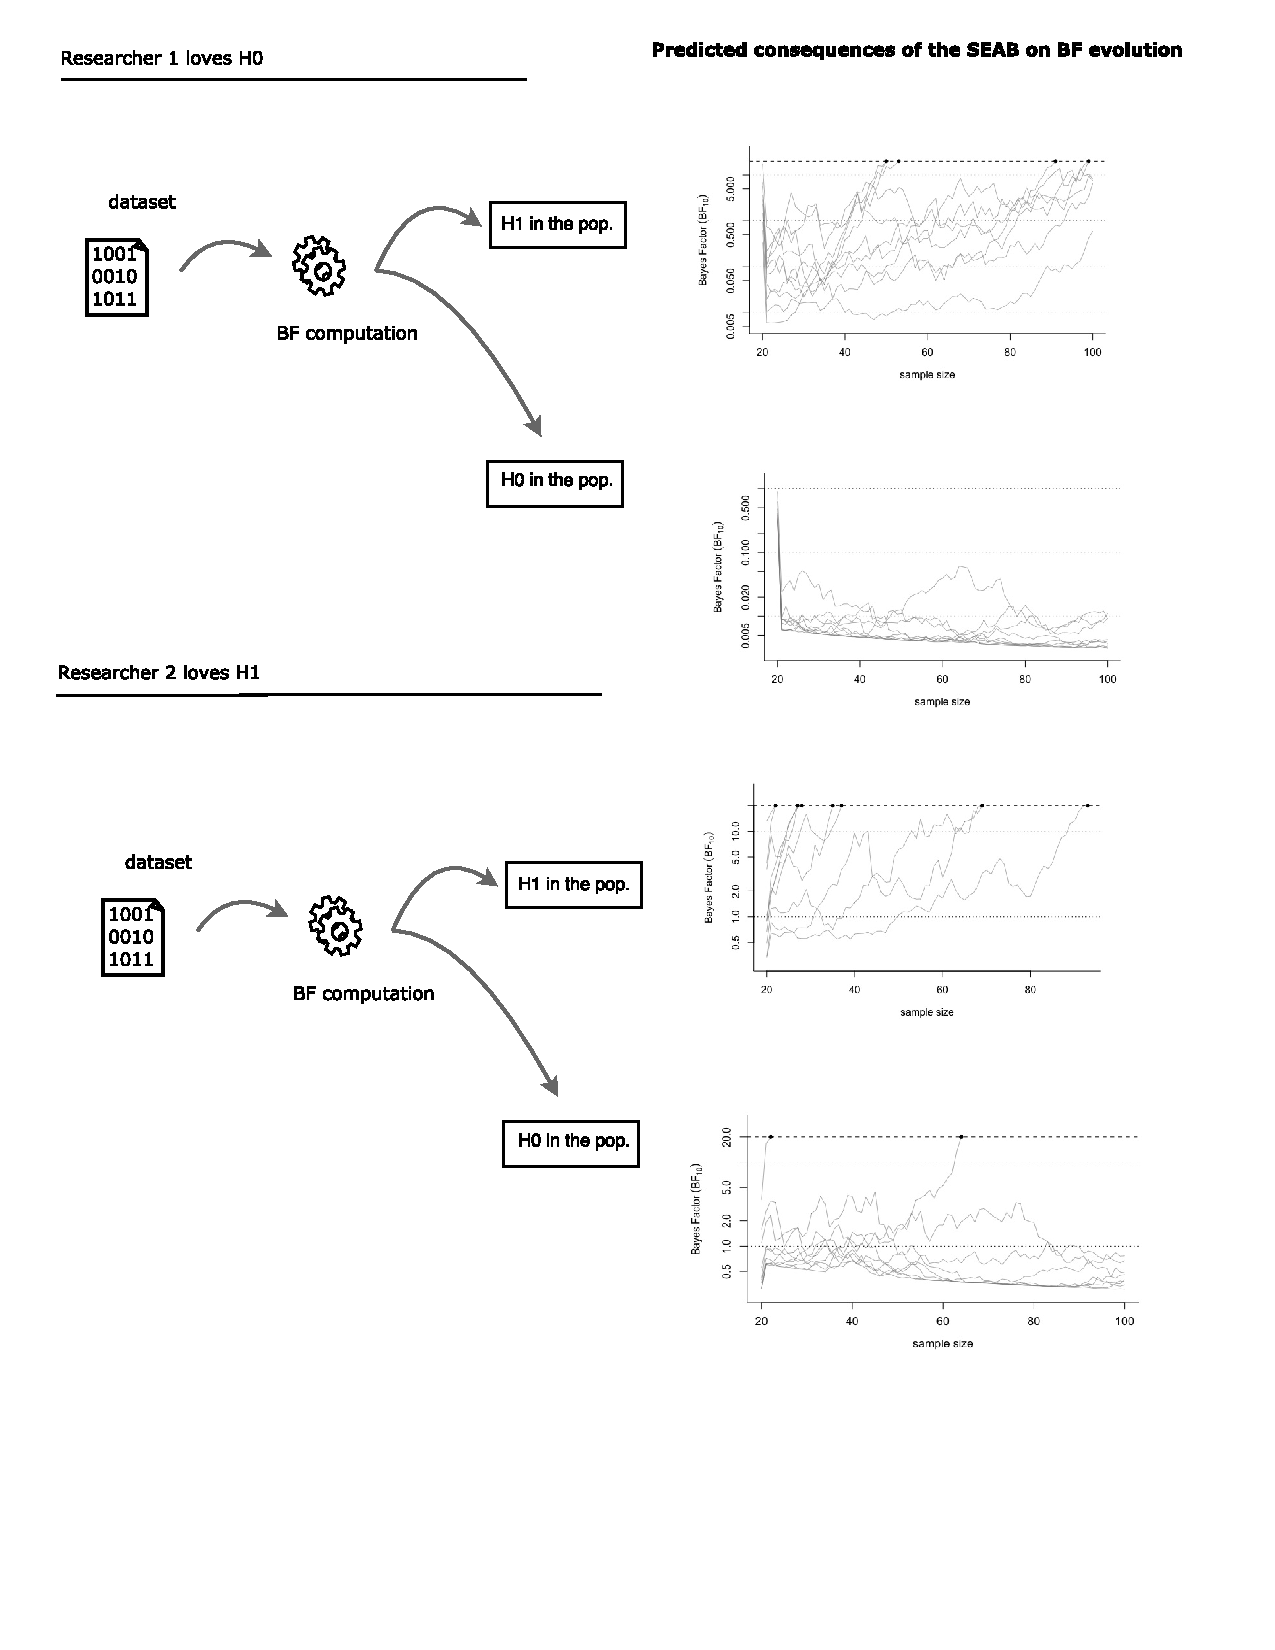
\includegraphics[width=0.8\textwidth]{figures/BFF_predictions.pdf}
  \label{fig:pred}
\end{figure}

In the current section we have presented how the knowledge of previous data can bias the data collection process and have also illustrated the predicted consequences of these biases on the evolution of sequentially computed Bayes Factors. In the next section we therefore focus on how to prevent these biases from happening. We suggest two ways of implementing analysis blinding as a precaution against experimenter biases during sequential testing, and present a proof of concept for an automated procedure that would ensure objectivity.

\section{Strengths and weaknesses of automation as compared to classical blinding}

\subsection{Solution 1: one analyst, one experimenter}

Double blinding advantages are well documented \citep{schulz_blinding_2002}. However although this procedure can minimise the experimenter effect, it is not always practicable. Experimenter blinding procedures are considered as the gold standard of procedures in many psychological fields. However much less attention has been given to analysis blinding. In the SBF procedure analysis blinding can take two different forms. First, analysis blinding can refer to a procedure ensuring that the person who analyses the data is blind to the hypotheses \citep{miller_blind_2011}, thus minimising intra-personal biases because the analyst has not particular interest in corroborating or disproving it. Second (and specific to sequential testing procedures), analysis blinding can refer to a procedure ensuring that the experimenter is blinded to the data analysis (minimising interpersonal biases).

Whilst not widespread in psychology due to the availability of materials and time constraints, the use of analysis blinding would help eliminate some of the biases identified in \cite{wicherts_degrees_2016}. In the SBF context, if the experimenter is not the data analyst, s·he can be blind to the evolution of the Bayes Factor until data collection stops. As a consequence, the specific SBF experimenter expectancy bias is avoided.

\subsection{Solution 2: one analyst-experimenter, "software-blinded"}

Another solution is to automate analysis blinding so that the data analyst and the experimenter (who can be the same person) are blind to BFs computed on previous sets of observations. To illustrate this idea we wrote a short function allowing SBF to be run for two-independent groups comparisons \citep[as in][]{schonbrodt_sequential_2017}. The user can set the \texttt{blind} argument to \texttt{TRUE} and be completely blind to the results of the SBF procedure. The only output is a sentence that either indicates to "continue" or to "stop" the recruitment, considering an a priori defined threshold (see \nameref{sec:supp} for code details). The advantage of this being a costless and ready-to-use solution.

Using this function we reanalysed a dataset issued from the reproducibility project \citep{open_science_collaboration_estimating_2015} and ran three analyses i) a classical SBF procedure, ii) an SBF procedure in which experimenter and participants errors were iteratively removed from the considered dataset, and iii) a SBF procedure in which errors as well as outliers were removed from the dataset. Results of the three procedures can be found in the \nameref{sec:supp}. We suggest combining automated data preprocessing with blind analyses in order to ensure objectivity during sequential testing.

\section{Limits}

We concede that automation of data analysis prevents one interesting advantage of sequential testing. This being that data collection can be stopped when the behaviour of data is unexpected, allowing the experimenter to rethink the experimental design or aim  before collecting more data \citep{lakens_performing_2014}. Depending on the confidence and expected familiarity with the data to be collected, the researchers have to choose between automated or "two-persons" analysis blinding. The first option is costless while the second one is more flexible. In any case, after performing SBF nothing prevents the researcher from performing additional analyses based on data specificities, taking care to record the exploratory nature of any such analyses. 

\section{Conclusions}

The current article proposes a straightforward approach for analysis blind designs when using sequential testing. Although the magnitude of intrapersonal and interpersonal biases is uncertain during data analysis and data collection, analysis blinding is a costless security likely to increase the transparency and reliability of data analysis. Due to its specific status, sequential testing could benefit from analysis blinding even more than traditional analysis methods. Analysis blinded sequential testing could improve hypothesis testing within the "costs and benefits trade-off" world of the researcher.

\section{Supplementary materials}\label{sec:supp}

Reproducible code and supplementary materials can be found on OSF: \url{osf.io/mwtvk
}.

\section{Acknowledgements}

We thank Hans Ijzerman for helpful comments on a previous version of this manuscript and Edward Collett for his help with manuscript English proof reading.

\bibliography{BBF}

\end{document}
